\section{Transaksjoner}
\begin{frame}{Hvorfor Transactions?}
    \begin{itemize}[<+->]
        \item Sammenfatte flere kommandoer til en transaksjon
        \item Passe på at alt eller ingenting blir utført
        \item Passe på at flere kommandoer ikke blandes med hverandre
    \end{itemize}
\end{frame}

\begin{frame}{ACID Prinsipper}
    \begin{itemize}[<+->]
        \item Atomicity: Alt eller ingenting blir utført.
        \item Consistency: Databasen går fra en gyldig til en gyldig status.
        \item Isolation: Parallele transaksjoner ser ikke hverandre.
        \item Durability: Resultater av en transaksjon blir ikke overskrevet av den neste transaksjonen.
    \end{itemize}
\end{frame}

\subsection*{Ting som kan gå galt}
\begin{frame}{}
    \begin{block}{Lost Update}
    To transaksjoner jobber på samme tall på samme tidspunkt og den ene overskrever den andres verdien.
    \end{block}
    \pause
    \begin{itemize}[<+->]
        \item Vi får samtidig 1.000 kr fra bestemoren (A) og betaler 100kr til hvem som helst (B)
        \item A leser verdien på kontoen (5000kr)
        \item B leser verdien på kontoen (5000kr)
        \item A legger til 1.000kr og skriver verdien tilbake til databasen (6000kr)
        \item B fjerner 100kr og skriver verdien tilbake til databasen (4900kr)
        \item B har overskrevet resultatet til A
    \end{itemize}
    
\end{frame}

\begin{frame}{}
    \begin{block}{Aborted Update}
    En kommando ikke blir tilbakegjort etter rollback.
    \end{block}
    \pause
    \begin{itemize}[<+->]
        \item A sender 100kr til B
        \item Banken fjerner 100kr fra kontoen til A
        \item Det skjer en feil når man gir 100kr til B
        \item Nå har A tapt 100kr, men B ikke fått 100kr
        \item Databasen må nå rette kontoen til A
    \end{itemize}
\end{frame}

\begin{frame}{}
    \begin{block}{Inconsistent Analysis}
    En kommando baserer seg på både gamle data og nye data samtidig.
    \end{block}
    \pause
    \begin{itemize}[<+->]
        \item Vi skal legge til en film og en screening i databasen
        \item I tillegg skal vi få en joined tabell med alle filmer og screenings til sammen
        \item Hvis man legger til film, kjører JOIN kommandoen og etterpå legger til screening, har vi \textit{inconsistent analysis}
        \item Kommandoen baserer informasjoner på gamle verdier (screening tabell) og nye verdier (film database) samtidig
        \item Enten gjør alle INSERT på begynnelsen eller på slutten
    \end{itemize}
\end{frame}

\subsection*{SQL Transaksjoner}
\begin{frame}[fragile]{Transaksjoner i SQL}
\begin{minted}{sql}
START TRANSACTION;      -- her starter transaksjonen
UPDATE bankaccount      -- ta 20kr fra en bankkonto 
SET money = money - 20  -- dette er ikke korrekt syntaks
WHERE customer = 42;
UPDATE bankaccount      -- gi de 20kr til en annen bankkonto
SET money = money + 20
WHERE customer = 20;
COMMIT;                 -- commit hvis alt gikk fint, ellers rollback
-- ROLLBACK
\end{minted}
\end{frame}

\subsection*{Begrep}
\begin{frame}
\begin{itemize}[<+->]
    \item Serialisability: To transaksjoner er serialisable dersom det finnes en rekkefølge de kan utføres uten at de ignorerer ACID-prinsippene
    \item Write lock: Variabel kan ikke endres, men verdien kan leses 
    \item Read lock: Variabel kan verken leses eller endres
    \item Two phase locking: Blokker alle variabler samtidig, frigir dem samtidig
\end{itemize}
\end{frame}

\subsection*{Waiting graph}
\begin{frame}{Finn rekkefølge for transaksjoner}
\begin{itemize}[<+->]
    \item Lag rettet graf med transaksjoner som noder
    \item A venter til B: $A \rightarrow B$ (retningen antiintuitiv)
    \item Finn en rekkefølge å gå gjennom nodene
    \item Hvis graf har sykler finnes ikke en sånn rekkefølge
    \item Fjern de eldste transaksjonene inntil ingen sykler er igjen
\end{itemize}
\end{frame}

\begin{frame}{Eksempel}
\begin{columns}
    \begin{column}{0.48\textwidth}
\begin{tikzpicture}[
    node distance=1.45cm, thick,
    main node/.style={circle, draw, font=\sffamily\bfseries}
]
    \node<-4>[main node] (1)                    {1};
    \node[main node,onslide=<8>{fill=black!60!green}] (3) [below left  of=1] {3};
    \node[main node,onslide=<7->{fill=black!60!green}] (4) [below right of=1] {4};
    \node[main node,onslide=<3->{fill=black!60!green}] (2) [above right of=4] {2};
    \node[main node,onslide=<4->{fill=black!60!green}] (6) [below right of=4] {6}; % <-4> forces an additional overlay in which node 2 disappears

    \path<1>[->] (1) edge (2)
        (4) edge (2)
        (6) edge (2);
    \path<-4>[->] (1) edge (3)
        (4) edge (1);
    \path<-5>[->] (3) edge (4);
\end{tikzpicture}
 \end{column}
    \begin{column}{0.48\textwidth}
\begin{itemize}
    \item<1-> Graf med fem noder 
    \item<2-> Transaksjon 2 venter på ingenting
    \item<3-> Marker transaksjon 2 som utført
    \item<4-> Marker transaksjon 6 som utført
    \item<5-> Funnet syklus, fjern eldeste transaksjon 1
    \item<6-> Transaksjon 4 venter på ingenting
    \item<7-> Marker transaksjon 4 som utført
    \item<8-> Marker transaksjon 3 som utført
\end{itemize}
 \end{column}
\end{columns}
\end{frame}

\subsection*{Spørretid}
\begin{frame}{Spørsmål?}
    \begin{figure}
        \centering
        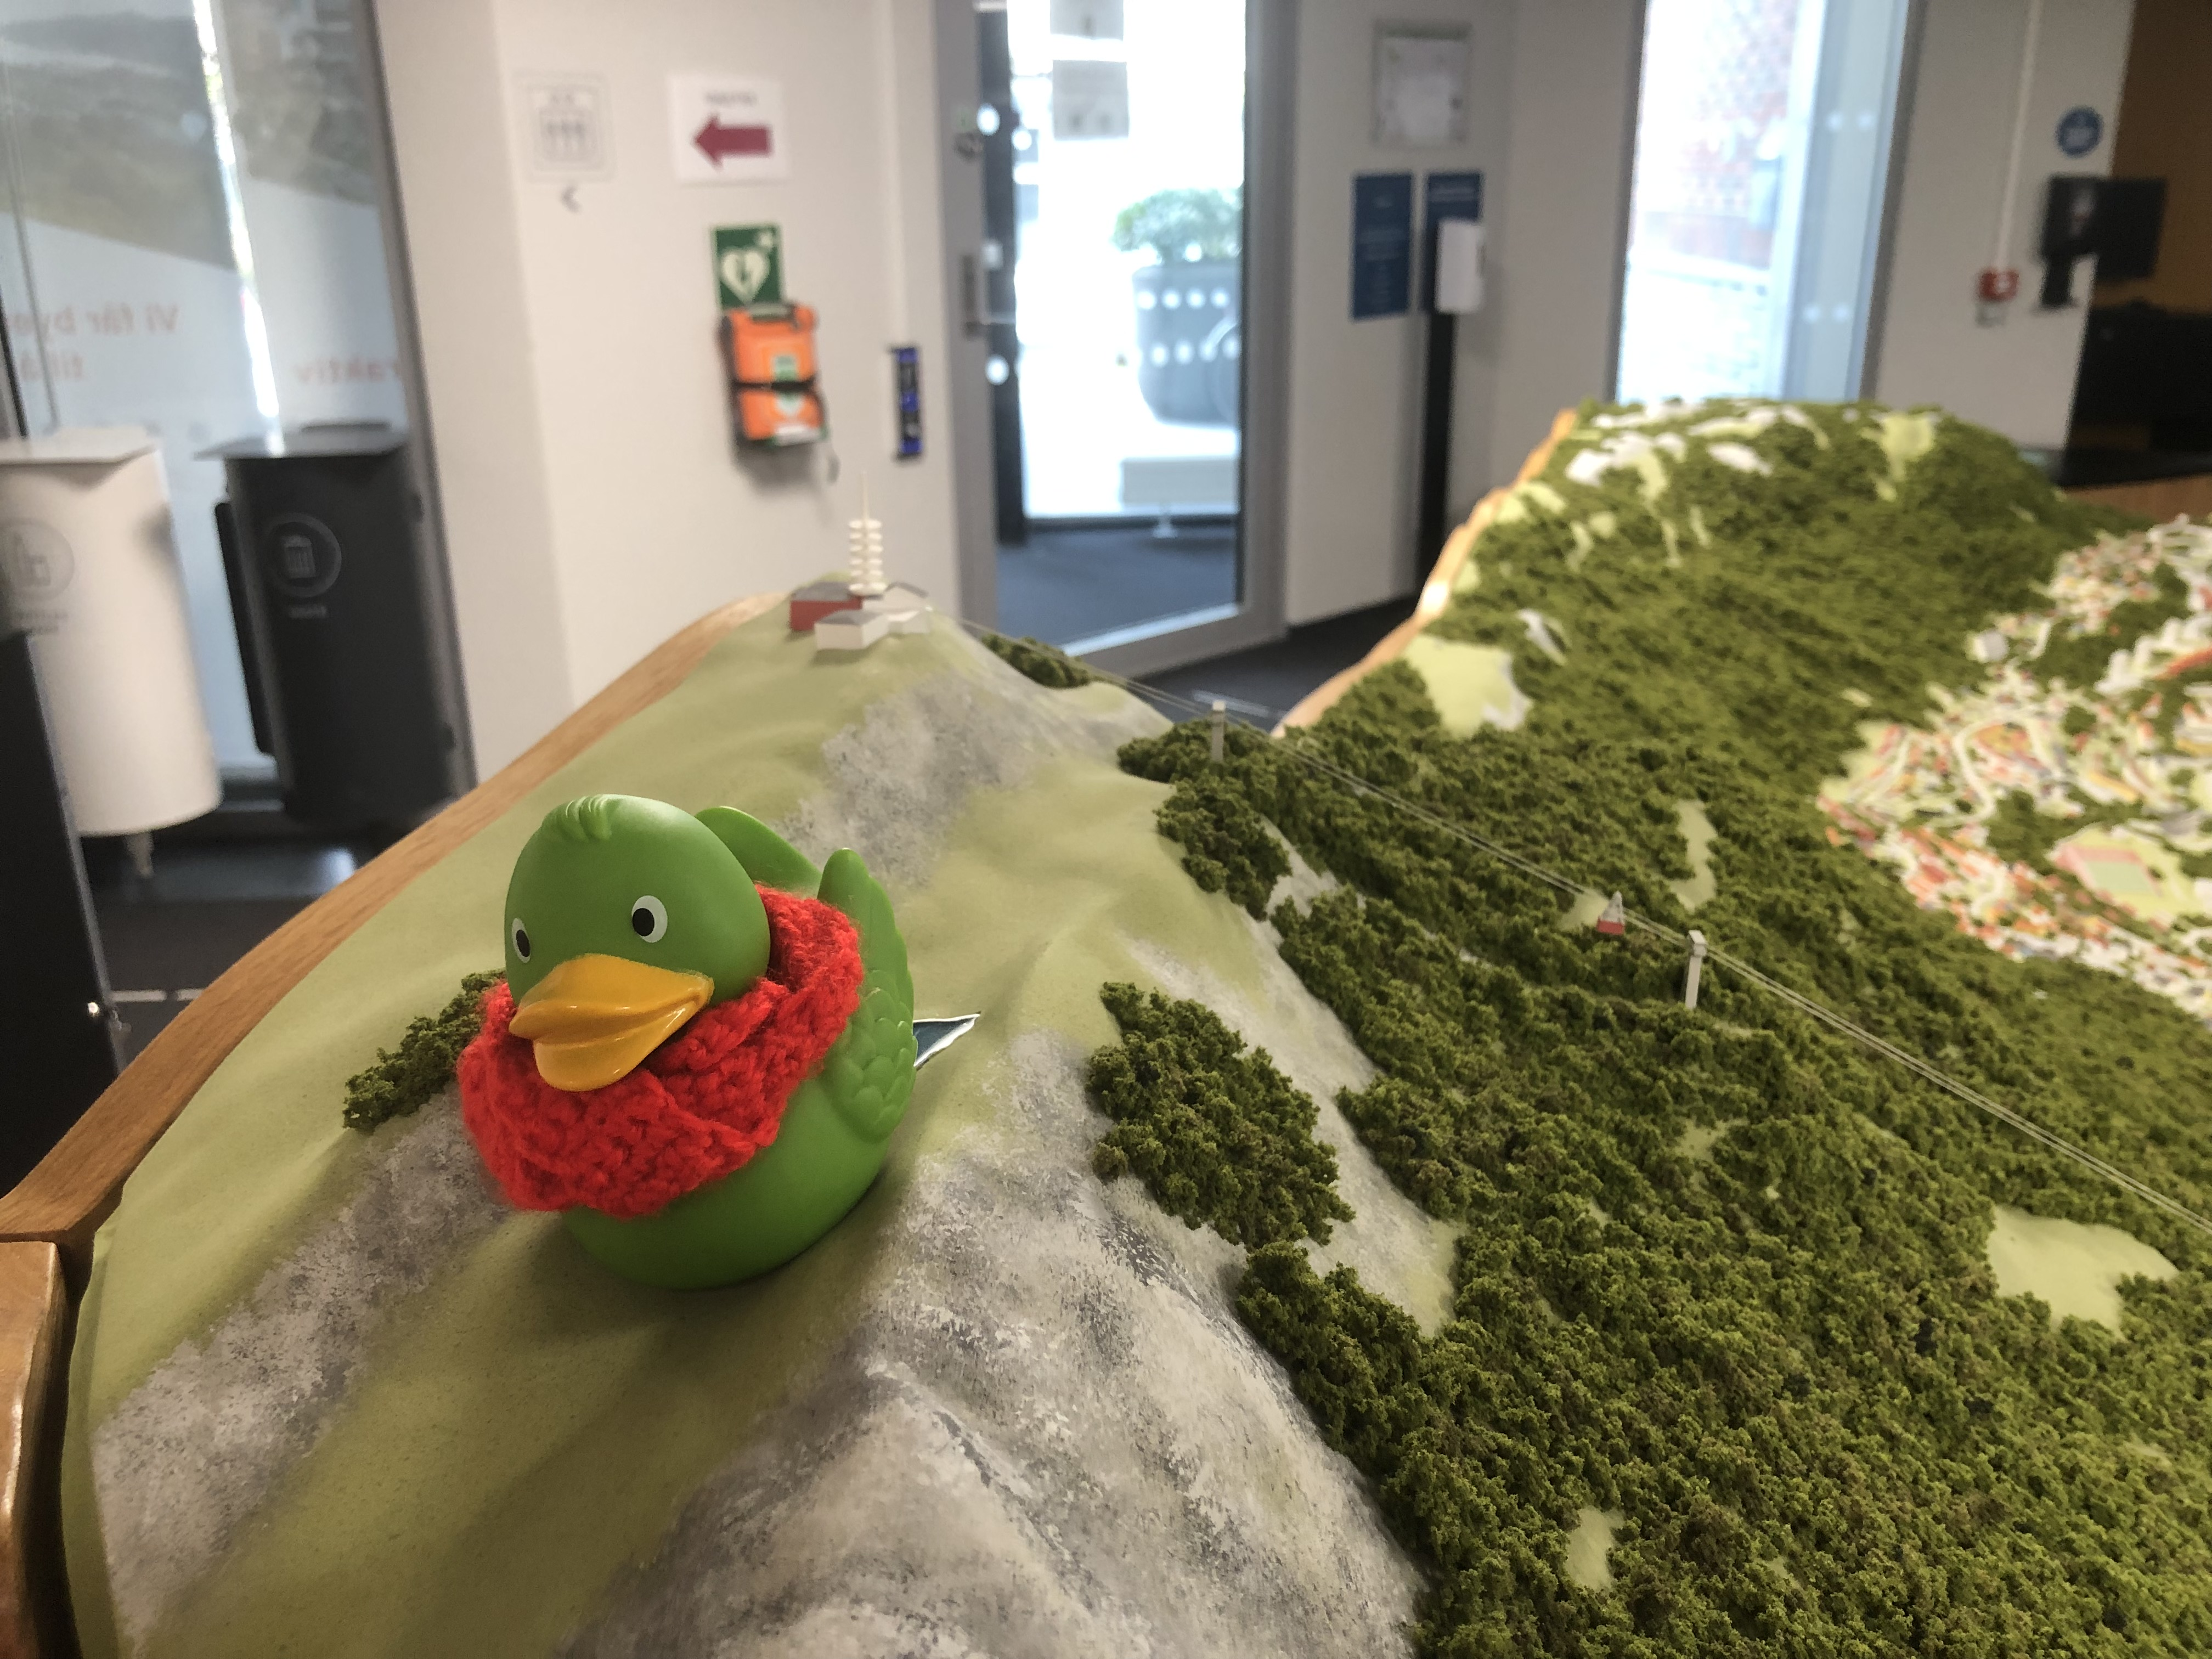
\includegraphics[height = 4.9cm]{images/guillaume11.jpg}
        \caption{Guillaume på Ulriken}
        \label{fig:guillaume11}
    \end{figure}
\end{frame}
